
從併發性的角度來看,\textbf{堆棧}是最簡單的數據結構之一。堆棧上的所有操作都處理頂部元素,因此(至少在概念上)需要保護一個位置以防止競爭。

C++標準庫提供了\texttt{std::stack}容器,可以將該容器作為一個起點。所有C++容器,都提供了弱線程安全。多個線程可以安全地訪問只讀容器,只要沒有線程調用非\texttt{const}函數,任意數量的線程都可以同時調用任何\texttt{const}方法。這聽起來很簡單,幾乎過於簡單,但這裡有一個問題。在最後一次修改和只讀的部分之間,必須存在某種同步,所有線程在內存柵欄之前執行,寫訪問並沒有真正完成。寫線程至少需要釋放內存,而讀線程必須獲取內存。任何強柵欄都可以工作,鎖也可以,但每個線程都必須邁出這一步。

\subsubsubsection{7.3.1\hspace{0.2cm}線程安全接口的設計}

現在,如果多個線程在修改堆棧,則需要更強的保證,那該怎麼辦?提供互斥鎖的最直接的方法,用鎖保護類的每個成員函數。這可以在應用程序級別完成,但是這樣的實現並不是強線程安全,並且很容易出錯。因為鎖與容器沒有關聯,也很難進行調試和分析。

更好的選擇是用自己的類包裝堆棧類:

\hspace*{\fill} \\ %插入空行
\noindent
\textbf{02\_stack.C}
\begin{lstlisting}[style=styleCXX]
template <typename T> class mt_stack {
	std::stack<T> s_;
	std::mutex l_;
	public:
	mt_stack() = default;
	void push(const T& v) {
		std::lock_guard g(l_);
		s_.push(v);
	}
	…
};
\end{lstlisting}

注意,可以使用繼承而不是封裝。這樣做會使\texttt{mt\_stack}的構造函數更簡單,只需要一個\texttt{using}語句。但是,使用公共繼承會公開基類\texttt{std::stack}的每個成員函數,若忘記包裝其中一個,代碼將直接調用未保護的成員函數。私有(或受保護的)繼承避免了這個問題,但會帶來其他風險。有些構造函數需要重新實現,例如:移動構造函數需要鎖定正在移動的堆棧,因此需要自定義實現。在沒有包裝器的情況下,公開其他幾個構造函數十分危險,因為它們會讀取或修改參數。總的來說,必須重寫每個構造函數,這樣比較安全。這與C++的建議是一致的,\textit{組合優於繼承}(\textit{prefer composition over inheritance})。

線程安全或多線程堆棧(就是\textit{mt}的意思)現在有了\textit{push}功能,並準備接收數據。現在,只需要逆操作\textit{pop}。當然可以按照前面的例子包裝\texttt{pop()},但這還遠遠不夠。STL堆棧使用三個獨立的成員函數從堆棧中刪除元素,\texttt{pop()}刪除了頂部元素,但沒有任何返回。所以想知道堆棧頂部是什麼,必須先使用\texttt{top()}。如果堆棧為空,那麼使用這兩種方法中的任何一個都會導致未定義行為,所以必須先使用\texttt{empty()}檢查結果。這裡需要包裝這三個方法,這裡先不展示。下面的代碼中,假設堆棧的所有成員函數都由一個鎖保護:

\begin{lstlisting}[style=styleCXX]
mt_stack<int> s;
… push some data on the stack …
int x = 0;
if (!s.empty()) {
	x = s.top();
	s.pop();
}
\end{lstlisting}

每個成員函數都是線程安全的,但在多線程上下文中完全沒用。堆棧可能在某一刻(碰巧使用\texttt{s.empty()}的那一刻)非空,但在下一刻(調用\texttt{s.top()}之前)就變成空的了,在此期間另一個線程可以刪除頂部的元素。

這可能是整本書最重要的內容了。為了提供可用的線程安全功能,在選擇接口時必須考慮線程安全,但不能在現有的設計上添加線程安全的特性。在進行設計時,必須考慮到線程安全。因為可以選擇在設計中提供某些保證和不變量,這些在併發程序中不可維護,例如:\texttt{std::stack}保證調用\texttt{empty()}是安全的,並返回false,這樣就可以安全地調用\texttt{top()},只要在這兩個調用間不做其他的堆棧操作就好。在多線程程序中,沒有特別好的方法來履行這種承諾。

幸運的是,由於正在編寫自己的包裝器類,所以不需要逐個使用包裝類的接口。那麼,應該怎麼做呢?顯然,整個\texttt{pop}操作是一個成員函數,應該從堆棧中刪除頂部元素,並將其返回給調用者。問題是當堆棧為空時該做什麼?有多種選擇。可以返回一對值和一個布爾標誌,該標誌指示堆棧是否為空(這種情況下,該值必須有默認構造)。也可以單獨返回布爾值,並通過引用傳遞該值(如果堆棧為空,則該值保持不變)。在C++17中,解決方案是返回\texttt{std::optional},如以下代碼所示。它非常適合持有可能並不存在的值:

\hspace*{\fill} \\ %插入空行
\noindent
\textbf{02\_stack.C}
\begin{lstlisting}[style=styleCXX]
template <typename T> class mt_stack {
	std::stack<T> s_;
	std::mutex l_;
	public:
	std::optional<T> pop() {
		std::lock_guard g(l_);
		if (s_.empty()) {
			return std::optional<T>(std::nullopt);
		} else {
			std::optional<T> res(std::move(s_.top()));
			s_.pop();
			return res;
		}
	}
};
\end{lstlisting}

將元素從堆棧中彈出的整個操作現在都受到鎖的保護,這個接口是事務性的。每個成員函數將對象從一個已知狀態轉到另一個已知狀態。

如果對象必須轉換到一些中間狀態,比如使用\texttt{empty()}之後,並在使用\texttt{pop()}之前的狀態,這些狀態必須對使用者不可見。相反,向使用者呈現的是原子事務。要麼返回頂部的元素,要麼通知調用者不能進行該操作,這確保了程序的正確性。現在,來看看性能。

\subsubsubsection{7.3.2\hspace{0.2cm}使用互斥的性能}

堆棧的性能如何?假設每個操作從開始到結束都是鎖定的,那就不要對堆棧成員函數的性能有什麼期待。最好的情況下線程都將串行地執行堆棧操作,實際中鎖應該會帶來一些額外的開銷。如果要比較多線程堆棧和普通\texttt{std::stack}的性能,可以在基準測試中進行對比。

為了簡化基準測試,可以選擇在\texttt{std::stack}上實現單線程的非阻塞包裝器,該包裝器提供與\texttt{mt\_stack}相同的接口。注意,不能僅通過\texttt{push}堆棧來進行基準測試,這樣基準測試可能會將內存耗盡。類似地,無法可靠地對\texttt{pop}操作進行基準測試,除非想測量從空堆棧彈出的耗時。如果基準測試運行的時間足夠長,就必須將\texttt{push}和\texttt{pop}結合起來。最簡單的基準測試可以是這樣的:

\hspace*{\fill} \\ %插入空行
\noindent
\textbf{02\_stack.C}
\begin{lstlisting}[style=styleCXX]
mt_stack<int> s;
void BM_stack(benchmark::State& state) {
	const size_t N = state.range(0);
	for (auto _ : state) {
		for (size_t i = 0; i < N; ++i) s.push(i);
		for (size_t i = 0; i < N; ++i)
		benchmark::DoNotOptimize(s.pop());
	}
	state.SetItemsProcessed(state.iterations()*N);
}
\end{lstlisting}

多線程時,有可能在堆棧為空時進行\texttt{pop()}操作。對於處於設計階段的堆棧來說,這是可能現實的。此外,由於基準測試提供了真實應用程序中數據結構性能的近似值,其中的差異可以忽略。不過,為了獲得更精確的測量值,必須模擬應用程序,並執行真實的\texttt{push}和\texttt{pop}操作序列。結果應該是這樣的:

%\hspace*{\fill} \\ %插入空行
\begin{center}
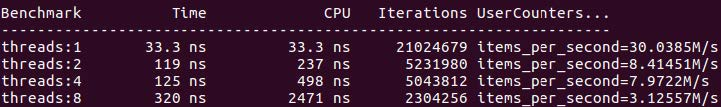
\includegraphics[width=0.9\textwidth]{content/2/chapter7/images/3.jpg}\\
圖7.3 - 鎖棧——使用互斥鎖——的性能
\end{center}

注意這裡的“item”是“push後面跟著pop”的操作,所以“items per second”的值顯示了每秒鐘可以通過堆棧發送多少數據。為了進行比較,沒有鎖的堆棧在單個線程上的執行速度,要比使用互斥鎖快10倍多:

%\hspace*{\fill} \\ %插入空行
\begin{center}
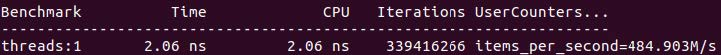
\includegraphics[width=0.9\textwidth]{content/2/chapter7/images/4.jpg}\\
圖7.4 - \texttt{std::stack}的性能(與圖7.3相比)
\end{center}

使用互斥對象實現的堆棧性能相當差。但不要急於設計一些聰明的線程安全堆棧,現在還不需要。這時,應該問的第一個問題是,這是怎麼回事?應用程序如何處理堆棧上的數據?如果每個數據元素都需要耗時幾秒鐘模擬一個參數,那麼堆棧的速度就不重要了。另外,如果堆棧位於某些實時事務處理系統的核心,那麼其速度可能是整個系統性能的關鍵。

順便說一下,結果可能與其他數據結構類似,如鏈表、雙端隊列、隊列和樹。其中,單個操作要比對互斥鎖的操作快得多。但是,在嘗試改進性能之前,必須準確地瞭解應用程序需要什麼樣的性能。

\subsubsubsection{7.3.3\hspace{0.2cm}不同的性能需求}

本章的其餘部分中,假設數據結構的性能在應用程序中很重要。現在,可以來聊聊最快的堆棧實現了吧?還沒到那個時候。還需要考慮使用的模型,該如何處理堆棧,以及什麼才是需要加速的東西。

互斥鎖堆棧性能較差的關鍵原因是,速度基本上受到互斥鎖的限制,對堆棧操作進行基準測試幾乎與對互斥鎖的鎖定和解鎖進行基準測試結果相同。提高性能的一種方法是改進互斥鎖的實現,或者使用另一種同步方案。另一種方法是少使用互斥鎖,這需要重新設計客戶端代碼。

例如,使用者通常有多個必須壓入堆棧的項。類似地,使用者可以一次從堆棧中彈出幾個元素並進行處理。這種情況下,可以使用數組或容器來實現批量推送或批量彈出,以便一次從堆棧中複製多個元素。由於鎖定的開銷很大,可以用鎖定/解鎖操作在堆棧上一次性推入1024個元素,這樣就比用鎖逐個推入元素來的快,基準測試也反映了這一點:

%\hspace*{\fill} \\ %插入空行
\begin{center}
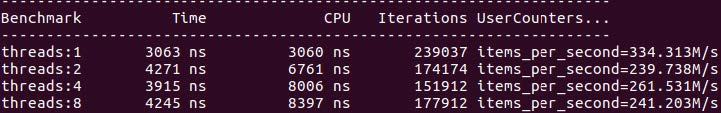
\includegraphics[width=0.9\textwidth]{content/2/chapter7/images/5.jpg}\\
圖7.5 - 批處理堆棧操作的性能(每個鎖1024個元素)
\end{center}

我們應該非常清楚這種方式可以做哪些事,不能做哪些事。若臨界區內的操作比鎖操作本身快得多,就該減少鎖的開銷,但不能鎖定操作的規模。此外,通過延長停留在臨界區的時間,迫使線程在鎖上等待更長時間。如果所有線程都嘗試訪問堆棧(這就是基準測試變得更快的原因),那沒問題。但若在應用程序中,線程主要是執行其他計算,只是偶爾訪問堆棧,那麼較長的等待可能會降低整體性能。為了明確地回答批量\texttt{push}和批量\texttt{pop}是否對性能有益,必須在更真實的環境中進行分析。

其他一些場景中,尋找更有限的、特定於應用程序的解決方案,可以獲得遠高於通用解決方案的改進,從而獲得的性能收益。單個線程將大量數據提前\texttt{push}到堆棧上,然後多個線程將數據從堆棧中刪除並處理,可能還會將更多數據\texttt{push}到堆棧上。這種情況可以實現解鎖的\texttt{push},只在單線程中的\texttt{push}中使用。雖然使用者的責任是,永遠不要在多線程中使用這個方法,但解鎖的堆棧比鎖定的堆棧快得多,因此這裡的複雜性是值得的。

更復雜的數據結構提供了各種各樣的使用模型,但即使是堆棧也可以使用,而不僅僅是簡單的\texttt{push}和\texttt{pop}。也可以查看頂部的元素而不刪除,\texttt{std::stack}提供了\texttt{top()}成員函數,但不是事務性的,所以必須創建自己的函數。其非常類似於事務性的\texttt{pop()}函數,只是不移除頂部的元素:

\hspace*{\fill} \\ %插入空行
\noindent
\textbf{02\_stack.C}
\begin{lstlisting}[style=styleCXX]
template <typename T> class mt_stack {
	std::stack<T> s_;
	mutable std::mutex l_;
	public:
	std::optional<T> top() const {
		std::lock_guard g(l_);
		if (s_.empty()) {
			return std::optional<T>(std::nullopt);
		} else {
			std::optional<T> res(s_.top());
			return res;
		}
	}
};
\end{lstlisting}

注意,為了允許只進行查找,這裡\texttt{top()}聲明為\texttt{const},這裡必須將互斥量聲明為\texttt{mutable}。這樣做時要小心,多線程程序的約定是遵循STL,只要不調用非\texttt{const}成員函數,所有\texttt{const}成員函數都可以安全地在多個線程上使用。這意味著\texttt{const}函數不會修改只讀對象,而可變數據成員違背了這個假設。至少,不應該表示對象的邏輯狀態。然後,在修改時應該避免競爭條件。互斥鎖必須滿足這兩個要求。

現在可以考慮不同的使用模式。某些應用程序中,數據\texttt{push}入堆棧,再從中\texttt{pop}出。其他情況下,堆頂元素可能需要在每次\texttt{push}和\texttt{pop}之間檢查多次。先關注後一種情況,而後再次檢查\texttt{top()}。這裡有一個明顯的低效行為,由於鎖的存在,只有一個線程可以讀取棧頂元素。但是讀取棧頂元素是一個非修改(只讀)操作。如果所有線程都這樣做,並且沒有線程同時嘗試修改堆棧,那麼就不需要鎖。但現在,它的性能與\texttt{pop()}一樣。

不能在\texttt{top()}中省略鎖,原因是不能確定另一個線程在同一時間沒有使用\texttt{push()}或\texttt{pop()}。但即使這樣,也不需要對\texttt{top()}進行兩次鎖定,它們可以同時進行,只有修改堆棧的操作需要鎖定。有一種類型的鎖提供這樣的功能,稱為\textbf{讀寫鎖}。任何數量的線程都可以獲得讀鎖,並且這些線程之間不會互相影響。但是,寫鎖只能由一個線程獲得,而且只有在沒有其他線程持有讀鎖的情況下才能獲取。在C++中,術語不同(但功能完全相同),讀線程使用共享鎖(同一個互斥對象上的共享鎖可以同時存在),但寫線程需要唯一鎖(給定的互斥對象上只能存在一個這樣的鎖)。如果另一個線程已經持有唯一鎖,那麼獲取共享鎖的嘗試將會阻塞。同樣,若另一個線程持有同一個互斥對象上的鎖,那麼獲取唯一鎖的嘗試將會阻塞。有了共享互斥鎖,就可以用需要的那種鎖來實現堆棧。\texttt{top()}使用了共享鎖後,任意數量的線程都可以同時執行,但\texttt{push()}和\texttt{pop()}需要唯一鎖:

\begin{lstlisting}[style=styleCXX]
template <typename T> class rw_stack {
	std::stack<T> s_;
	mutable std::shared_mutex l_;
	public:
	void push(const T& v) {
		std::unique_lock g(l_);
		s_.push(v);
	}
	std::optional<T> pop() {
		std::unique_lock g(l_);
		if (s_.empty()) {
			return std::optional<T>(std::nullopt);
		} else {
			std::optional<T> res(std::move(s_.top()));
			s_.pop();
			return res;
		}
	}
	std::optional<T> top() const {
		std::shared_lock g(l_);
		if (s_.empty()) {
			return std::optional<T>(std::nullopt);
		} else {
			std::optional<T> res(s_.top());
			return res;
		}
	}
};
\end{lstlisting}

但基準測試顯示,使用\texttt{top()}的性能即使在讀寫鎖下也不會改變:

%\hspace*{\fill} \\ %插入空行
\begin{center}
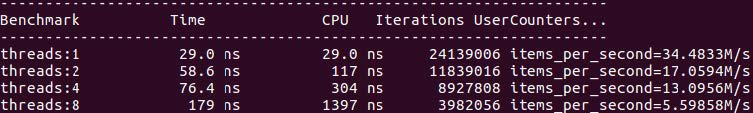
\includegraphics[width=0.9\textwidth]{content/2/chapter7/images/6.jpg}\\
圖7.6 - 使用\texttt{std::shared\_mutex}棧的性能——只讀操作
\end{center}

與普通互斥鎖相比,唯一鎖的性能下降得更厲害:

%\hspace*{\fill} \\ %插入空行
\begin{center}
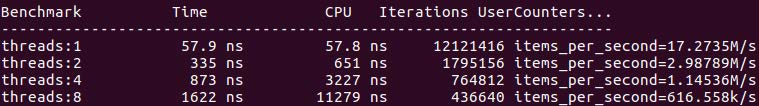
\includegraphics[width=0.9\textwidth]{content/2/chapter7/images/7.jpg}\\
圖7.7 - 使用\texttt{std::shared\_mutex}棧的性能——寫入操作
\end{center}

將圖7.6和7.7與圖7.4中的測試值進行比較,可以看到讀寫鎖並沒有任何改進。這個結論並不普遍,因為不同互斥量的性能取決於實現和硬件。然而,更復雜的鎖,比如共享互斥鎖,會比簡單鎖有更多的開銷。它們的目標程序不同的,若臨界區內的操作花費的時間非常久多(比如,毫秒而不是微秒),並且大多數線程執行只讀代碼,那麼就沒必要鎖定只讀線程將。

觀察更長的臨界段是非常重要的。如果堆棧元素較大,並且複製的代價非常高,那麼與複製大對象的代價相比,鎖的性能就不重要了。假設總體目標是使程序快速,而不是展示可擴展的堆棧實現,這裡將通過消除昂貴的複製,並使用指針堆棧來優化整個應用程序。

儘管讀寫鎖遇到了挫折,但我們正確的走在實現更高效應用的路上。在進行設計之前,我們必須更詳細地瞭解每個堆棧操作的作用,以及在每個步驟中必須避免可能出現的數據競爭。

\subsubsubsection{7.3.4\hspace{0.2cm}堆棧性能詳情}

在嘗試提高線程安全堆棧(或其他數據結構)的性能(不是簡單的鎖保護實現)時,必須詳細瞭解每個操作所涉及的步驟,以及如何與在不同線程上與其他操作交互。本節的目標不是更快的堆棧,而是進行分析。因為底層步驟在許多數據結構中都有,這裡我們從\texttt{push}操作開始。大多數堆棧實現都是建立在類似數組的容器上,所以可以把堆棧的頂部看作是一個連續的內存塊:

%\hspace*{\fill} \\ %插入空行
\begin{center}
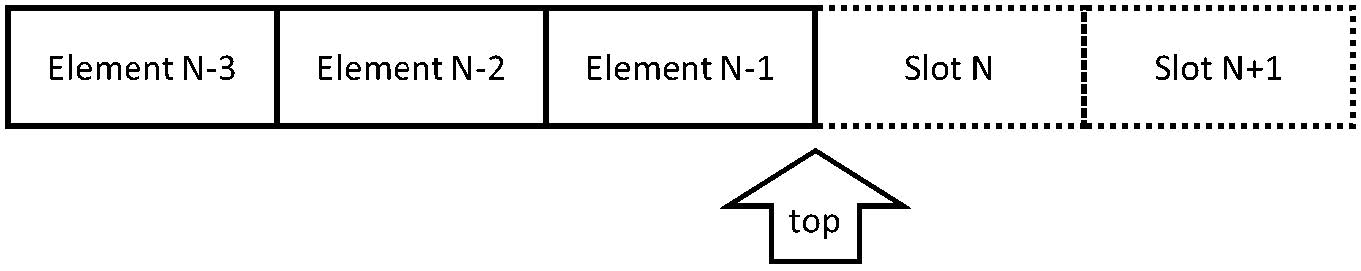
\includegraphics[width=0.9\textwidth]{content/2/chapter7/images/8.jpg}\\
圖7.8 - 棧頂的\texttt{push}操作
\end{center}

堆棧上有N個元素,所以元素計數也是下一個元素的槽索引。\texttt{push}操作必須將\texttt{top}索引(也是元素計數)從N增加到N+1,以保留槽位,然後在槽位N中構造新元素。注意,這個\texttt{top}索引是執行\texttt{push}操作的線程。只要索引增量操作是線程安全的,那麼只有一個線程可以看到索引的值。執行\texttt{push}操作的第一個線程將頂部索引提升到N+1,並保留第N個槽位,下一個線程將索引增加到N+2,並保留第N+1個槽位,以此類推。這裡的關鍵是插槽不存在競爭,因為只有一個線程可以獲得特定的插槽,因此可以在那裡構造對象,而不會有其他線程進行幹擾。

這就為\texttt{push}操作提供了非常簡單的同步方案,所需要的只是棧頂索引是原子值:

\begin{lstlisting}[style=styleCXX]
std::atomic<size_t> top_;
\end{lstlisting}

\texttt{push}操作會自動增加這個索引,然後在數組槽中構造新元素(按索引的舊值索引):

\begin{lstlisting}[style=styleCXX]
const size_t top = top_.fetch_add(1);
new (&data[top]) Element(… constructor arguments … );
\end{lstlisting}

同樣,不需要保護構造步驟。要讓\texttt{push}操作線程安全,只需要原子索引即可。如果使用數組作為堆棧內存,也沒問題。若使用\texttt{std::deque}這樣的容器,就不能簡單地在內存上構造一個新元素了,這裡需要使用\texttt{push\_back}來更新容器,而且這個操作不是線程安全的,即\texttt{deque}可能不需要分配更多的內存。由於這個原因,不在鎖管理下數據結構通常需要自己管理內存。說到內存,到目前為止,我們假設數組有足夠的空間添加更多的元素,並且不會耗盡內存。這裡繼續堅持這個假設。

現在,在特定情況下實現線程安全的\texttt{push}操作,是一種非常高效的方式。多個線程會將數據推送到堆棧上,但在所有的\texttt{push}操作完成之前不能讀取數據。

若有一個堆棧,其中已經有了元素,需要彈出它們(並且沒有添加更多的新元素),也可以使用相同的方法。圖7.8也適用於這種場景:一個線程自動減少\texttt{top}計數,然後返回\texttt{top}元素:

\begin{lstlisting}[style=styleCXX]
const size_t top = top_.fetch_sub(1);
return std::move(data[top]);
\end{lstlisting}

原子自減保證了只有一個線程可以訪問頂部元素的數組槽。當然,這隻在堆棧不是空的情況下才有效。可以將頂部元素的索引從無符號改為有符號整數,當索引為負時,就知道堆棧為空了。

這也是在非常特殊的條件下,實現線程安全\texttt{pop}操作的一種有效方式。堆棧已經填充,並且沒有添加新元素。本例中,還需要知道堆棧上有多少元素,因此可以避免彈出空堆棧。

一些特定的應用程序中,這可能是有價值的。若堆棧由多個線程填充,沒有任何彈出,並且在程序中有明確定義的點,從添加數據切換到刪除數據,就存在一個很好的解決方案。不過,現在我們想繼續討論更一般的情況。

但高效的\texttt{push}操作對於從棧中讀取數據毫無幫助,需要考慮如何實現彈出頂部元素的操作。我們有頂部索引,但它只表明當前有多少元素正在構造。沒有提到構造最後一個元素的位置(圖7.9中的元素N-3):

%\hspace*{\fill} \\ %插入空行
\begin{center}
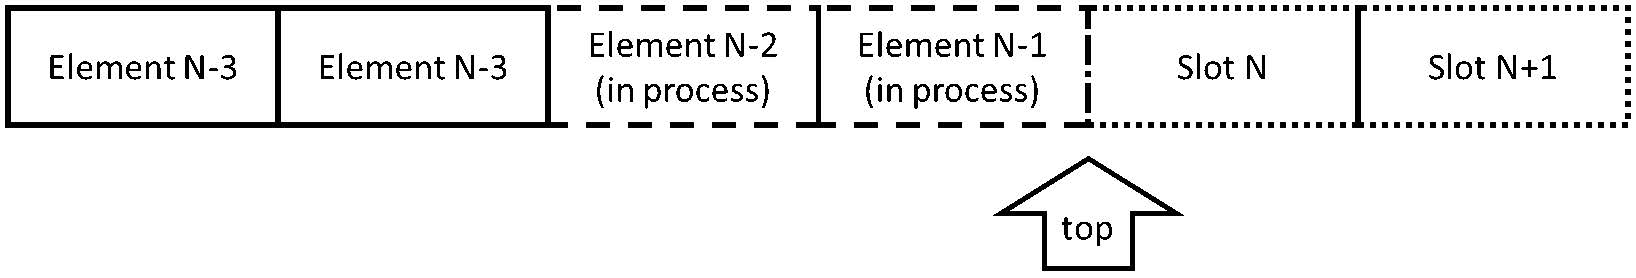
\includegraphics[width=0.9\textwidth]{content/2/chapter7/images/9.jpg}\\
圖7.9 - \texttt{push}和\texttt{pop}操作棧的頂部
\end{center}

當然,執行\texttt{push}和構造操作的線程,知道什麼時候完成構造。也許需要的是另一個計數,顯示有多少元素完成構造。唉……要是有那麼簡單就好了。圖7.9中,假設線程A正在構造元素N-2,而線程B正在構造元素N-1。顯然,線程A是第一個增加頂索引的。但這並不意味著它也是第一個完成\texttt{push}操作的,也許線程B可以先完成構造。現在,堆棧上最後一個構造元素的索引是N-1,所以可以將構造計數提升到N-1(注意,跳過了仍在構造中的元素N-2)。現在想要彈出頂部元素。沒問題,因為元素N-1已經準備好了,所以可以把它返回給使用者,並從堆棧中移除,構造計數現在減少到N-2。接下來應該彈出哪個元素?元素N-2沒有準備好,但堆棧中沒有任何警告。只有一個完成元素的計數,它的值是N-1。現在,在堆棧上構造新元素的線程和試圖彈出新元素的線程之間,出現了數據競爭。

即使沒有競爭,還有另一個問題:只彈出元素N-1,這在當時是正確的做法。但是,當線程C請求了一個\texttt{push}時,應該使用哪個插槽?如果使用槽位N-1,則可能會覆蓋線程A當前訪問的元素。如果使用槽位N,當所有的操作都完成,數組中就會出現一個洞。頂部的元素是N,但下一個元素不是N-1,N-1已經彈出,必須跳過它。據結構沒有告訴我們必須這樣做。

可以跟蹤哪些元素是存在,哪些元素是洞,但這些問題會將場面弄得越來越複雜(以線程安全的方式進行將需要額外的同步,這會降低性能)。另外,留下許多未使用的數組槽會浪費內存。可以嘗試為\texttt{push}堆棧的新元素重用已空閒的槽,但這時元素不再連續存儲,原子頂部計數不再工作,整個結構類似於一個鏈表。如果認為鏈表是實現線程安全堆棧的好方法,在本章後面的內容中會看到如何實現線程安全的鏈表。

在設計上,必須暫停深入研究實現細節,並再次檢查解決問題的更一般方法。需要由兩個步驟完成:從對堆棧實現細節的更深入理解中總結出結論,並進行性能估計,以大致瞭解哪些解決方案可能會帶來性能上的改進。我們先從後者開始。

\subsubsubsection{7.3.5\hspace{0.2cm}同步方案的性能評估}

我們第一次嘗試在沒有鎖的情況下實現一個堆棧,也產生了一些有趣的解決方案,但並沒有通用的解決方案。在花更多的時間構建一個複雜的設計之前,應該試著評估其比基於鎖的設計,更有效率的可能性有多大。

當然,這看起來像是循環推理。為了估計性能,必須首先對一些東西進行評估。但是我們不想浪費時間進行復雜的設計,所以才需要進行性能評估。

幸運的是,我們可以參考前面觀察的結果。併發數據結構的性能,很大程度上取決於併發訪問多少共享變量。假設可以想出一種聰明的方法,用一個原子計數器來實現堆棧。可以合理地假設,每次\texttt{push}和\texttt{pop}都必須對這個計數器進行至少一次原子遞增或遞減操作(除非正在進行批處理操作)。如果將單線程堆棧上的\texttt{push}和\texttt{pop}與共享原子計數器上的原子操作結合起來進行基準測試,可以得到一個合理的性能評估。因為沒有同步,所以必須為每個線程使用單獨的堆棧,以避免條件競爭:

\begin{lstlisting}[style=styleCXX]
std::atomic<size_t> n;
void BM_stack0_inc(benchmark::State& state) {
	st_stack<int> s0;
	const size_t N = state.range(0);
	for (auto _ : state) {
		for (size_t i = 0; i < N; ++i) {
			n.fetch_add(1, std::memory_order_release);
			s0.push(i);
		}
		for (size_t i = 0; i < N; ++i) {
			n.fetch_sub(1, std::memory_order_acquire);
			benchmark::DoNotOptimize(s0.pop());
		}
	}
	state.SetItemsProcessed(state.iterations()*N);
}
\end{lstlisting}

\texttt{st\_stack}是堆棧包裝器,提供的接口與基於鎖的\texttt{mt\_stack}相同,但不使用鎖。實際表現會稍微慢一些,因為堆棧頂部在線程之間共享,但這將會是對上面實現的評估:任何真正線程安全的實現,都不太可能比這個基準測試的性能更好。那用什麼來比較結果呢?圖7.3中基於鎖的堆棧基準展示了堆棧的性能,在線程上每秒進行30M次\texttt{push/pop}操作,在8個線程上每秒進行3.1M的\texttt{push/pop}操作。在沒有鎖的情況下,堆棧的基線性能大約是每秒\texttt{485M}個操作(圖7.4)。在同一臺機器上,使用單個原子計數器進行性能評估,結果如下:

%\hspace*{\fill} \\ %插入空行
\begin{center}
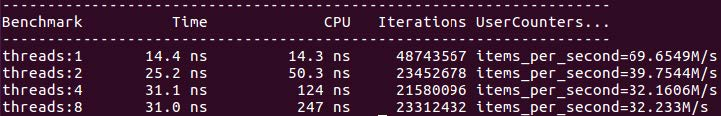
\includegraphics[width=0.9\textwidth]{content/2/chapter7/images/10.jpg}\\
圖7.10 - 性能評估——使用單個原子計數器的堆棧
\end{center}

結果看起來很複雜。即使在最優條件下,堆棧性能也不會改變。同樣,這主要是因為測試的是一堆小元素。因為多個線程可以同時複製數據,如果元素很大,且複製成本很高,就會看到擴展的性能。如果複製數據變得非常昂貴,需要很多線程來完成它,最好使用指針堆棧,從而不用複製任何數據。

另一方面,原子計數器要比基於互斥鎖的堆棧快得多。當然,這是上面的評估,但它表明無鎖堆棧存在一些可能性。然而,基於鎖的堆棧也是如此。當需要鎖定非常小的臨界區時,有比\texttt{std::mutex}更高效的鎖。實現自旋鎖後(已經在第6章中看到過一個這樣的鎖),並在基於鎖的堆棧中使用這個自旋鎖,與圖7.2不同,會得到如下的結果:

%\hspace*{\fill} \\ %插入空行
\begin{center}
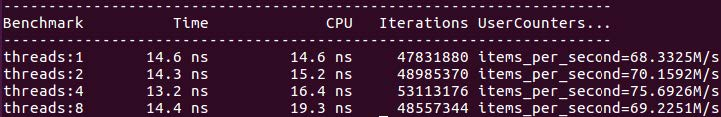
\includegraphics[width=0.9\textwidth]{content/2/chapter7/images/11.jpg}\\
圖7.11 - 基於自旋鎖堆棧的性能
\end{center}

將這個結果與圖7.10進行比較,會得出非常令人沮喪的結果,我們已經想不出一個比簡單自旋鎖更好的無鎖設計。某些情況下,自旋鎖的性能優於原子增量的原因,與不同的原子指令在特定硬件上的相對性能有關。所以這裡,不應該對此過度解讀。

可以嘗試用原子交換或比較-交換代替原子增量來完成評估測試。隨著瞭解了更多關於設計線程安全數據結構的知識,還將瞭解到有哪些同步協議可能有用,以及應該在評估中加入哪些操作。此外,如果使用特定的硬件,應該運行簡單的基準來確定哪些操作在該硬件上更高效。目前,所有的結果都是在基於x86的硬件上獲得的。如果在專門為HPC應用程序設計的基於ARM的大型服務器上運行相同的評估測試,會得到非常不同的結果。基於鎖的堆棧的基準測試結果如下所示:

%\hspace*{\fill} \\ %插入空行
\begin{center}
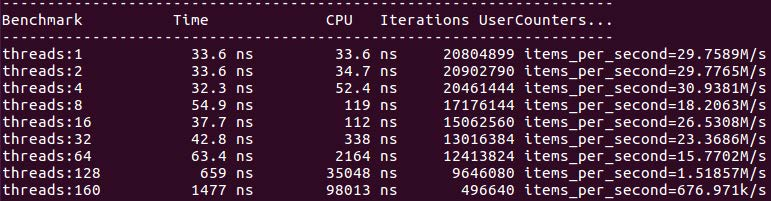
\includegraphics[width=0.9\textwidth]{content/2/chapter7/images/12.jpg}\\
圖7.12 - 基於鎖的堆棧在ARM HPC系統上的性能
\end{center}

ARM系統通常比x86系統有更多的內核,而單個內核的性能較低。這個特定系統的兩個物理處理器上有160個核,當程序在兩個CPU上運行時,鎖的性能會顯著下降。對無鎖堆棧性能上限的評估應該使用比較-交換指令來完成,而不是使用原子增量(後者在這些處理器上的效率特別低)。

\hspace*{\fill} \\ %插入空行
\begin{center}
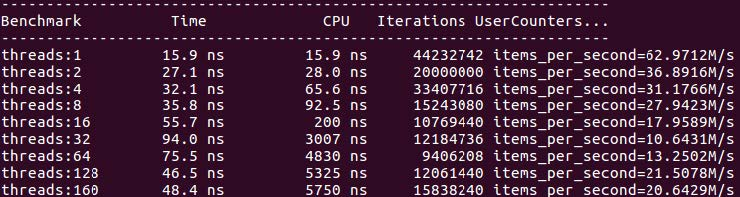
\includegraphics[width=0.9\textwidth]{content/2/chapter7/images/13.jpg}\\
圖7.13 - 堆棧中CAS操作的性能評估(ARM處理器)
\end{center}

根據圖7.13中的評估,對於大量的線程,可能有比基於鎖的堆棧更好的方法。我們將繼續努力開發一個無鎖堆棧,原因有二:首先,這種努力最終會在某些硬件上得到回報。其次,這個設計的基本元素將在許多其他數據結構中看到,並且堆棧可以提供了一個簡單的測試用例進行學習。

\subsubsubsection{7.3.6\hspace{0.2cm}無鎖的堆棧}

既然已經決定嘗試,並超越一個簡單的基於鎖的實現,需要考慮一下從\texttt{push}和\texttt{pop}操作本身的探索中獲得的經驗。每一個操作都很簡單,但兩者的交叉使用考究增加了複雜性。在多個線程上正確地同步生產者和消費者操作,要比只處理生產者或消費者操作困難得多。在設計自己的數據結構時請牢記,若應用程序允許對需要支持的操作進行類型限制,例如生產者和消費者在時間上是分開的,或者有一個生產者(或消費者)線程,那麼肯定可以為這些有限的操作,設計一個更快的數據結構。

假設需要一個完全通用的堆棧,生產者-消費者交互問題的本質可以通過一個簡單的例子來理解。同樣,假設堆棧是在數組或類似數組的容器之上實現,並且元素是連續存儲。假設堆棧上現在有N個元素,生產者線程P正在執行\texttt{push}操作,同時消費者線程C正在執行\texttt{pop}操作。結果是什麼?雖然很想嘗試一種無等待的設計(就像為僅消費者或僅生產者所做的那樣),但允許兩個線程在不等待的情況下進行的設計,都將打破對於元素如何存儲的假設。線程C必須等待線程P完成\texttt{push}操作,或者返回當前的頂部元素N。類似地,線程P必須等待線程C完成\texttt{push}操作,或者在槽N+1中構造一個新元素。如果兩個線程都沒有等待,那數組中就會出現空洞。最後一個元素的索引是N+1,但槽位N中沒有存儲任何內容,所以當從堆棧中彈出數據時,必須以某種方式跳過它。

看起來必須放棄無等待堆棧實現的想法,讓其中一個線程等待另一個線程完成它的操作。還必須處理當頂部索引為0,且消費者線程試圖進一步減少它時堆棧為空的可能性。當頂部索引指向最後一個元素時,數組的上界也會出現類似的問題,而生產者線程需要另一個槽。

這兩個問題都需要一個有界的原子自增操作。除非值等於指定值,才進行自增(或自減)。在C++中(或主流硬件上)沒有現成的原子操作,可以使用比較-交換(CAS)來實現,如下所示:

\begin{lstlisting}[style=styleCXX]
std::atomic<int> n_ = 0;
int bounded_fetch_add(int dn, int maxn) {
	int n = n_.load(std::memory_order_relaxed);
	do {
		if (n + dn >= maxn || n + dn < 0) return -1;
	} while (!n_.compare_exchange_weak(n, n + dn,
			std::memory_order_release,
			std::memory_order_relaxed));
	return n;
}
\end{lstlisting}

這是一個非常典型的例子,說明如何使用CAS操作實現一個複雜的無鎖原子操作:

\begin{enumerate}
\item 讀取變量的當前值。
\item 檢查必要的條件。本例中,驗證了增量不會給指定邊界外的值[0, maxn]。如果有界增量失敗,返回-1(通常,對於越界的情況,需要執行特定的操作)。
\item 如果當前值等於前面讀取的值,則會原子地將該值替換為所需的結果。
\item 如果步驟3失敗,則當前值已更新,請再次檢查它,並重復步驟3和4,直到成功。
\end{enumerate}

雖然這看起來像是一種鎖,但與鎖有一個根本的區別:CAS比較在一個線程上失敗的唯一原因是它在另一個線程上成功了(並且原子變量增加了),所以出現共享資源爭用時,至少有一個線程可以成功。

還有一個更重要的觀察結論,它常常決定了可擴展的實現和低效的實現之間的差別。CAS循環對大多數現代操作系統的調度算法非常不利,不能成功循環的線程會消耗更多的CPU時間,並將賦予更高的優先級。這與想要的完全相反,希望當前正在做有用工作的線程運行得更快。解決方案是讓一個線程在嘗試了幾次不成功的CAS之後生成調度,這可以通過系統調用來完成,但是C++有一個系統獨立的API,可以通過\texttt{std::this\_thread::yield()}進行。在Linux上,可以通過每隔幾次循環調用\texttt{nanosleep()}進行休眠,從而獲得儘可能短的時間(1納秒)來獲得更好的性能:

\begin{lstlisting}[style=styleCXX]
int i = 0;
while ( … ) {
	if (++i == 8) {
		static constexpr timespec ns = { 0, 1 };
		i = 0;
		nanosleep(&ns, NULL);
	}
}
\end{lstlisting}

同樣的方法也可以用於實現更復雜的原子事務,比如堆棧\texttt{push}和\texttt{pop},但必須先弄清楚需要哪些原子變量。對於生產者線程,需要數組中第一個空閒槽的索引。對於消費者線程,需要最後一個完成構造的元素的索引。這需要堆棧當前狀態的信息,並不允許數組中有“洞”出現:

%\hspace*{\fill} \\ %插入空行
\begin{center}
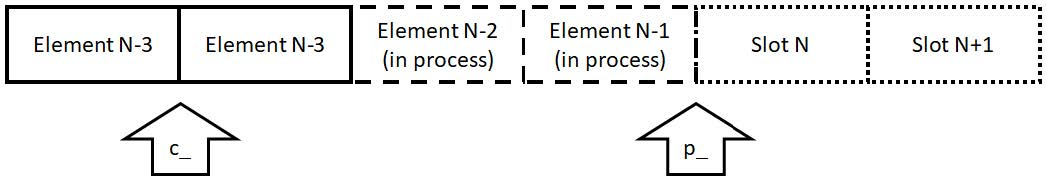
\includegraphics[width=0.9\textwidth]{content/2/chapter7/images/14.jpg}\\ 
圖7.14 —— 無鎖堆棧:\texttt{c\_}是最後一個完成構造的元素的索引,\texttt{p\_}是數組中第一個空閒槽的索引
\end{center}

如果兩個索引當前不相等,\texttt{push}和\texttt{pop}都不能進行。不同的計數意味著要麼構造一個新元素,要麼是複製當前頂部元素。在這種狀態下的堆棧修改都可能導致數組中出現空洞。

如果兩個索引相等,就可以繼續。為了執行\texttt{push}操作,需要自動增加生產者索引\texttt{p\_}(受數組當前容量限制)。然後,可以在剛才保留的槽中構造新元素(以舊的\texttt{p\_}值為索引)。然後,增加消費者索引\texttt{c\_},表示新元素對消費者線程可用。注意,另一個生產者線程可以在構造完成之前獲取下一個插槽,但必須等到所有新元素都構造好之後,才允許消費者線程彈出元素。這樣的實現是可能的,但更復雜,而且傾向於當前執行的操作。如果當前正在進行\texttt{push},則\texttt{pop}必須等待,但另一個\texttt{push}可以立即進行。結果很可能是,當所有消費者線程都在等待時,一堆\texttt{push}操作正在執行(如果\texttt{pop}操作正在進行,效果類似)。

\texttt{pop}的實現與此類似,只是首先遞減消費索引\texttt{c\_}以保留頂部的位置,然後遞減\texttt{p\_}從堆棧中複製或移動對象。

還需要學習一個技巧,那就是如何在原子上處理這兩個數。例如,線程必須等待兩個索引值相等,如何做到?如果以原子的方式讀取一個索引,然後以原子的方式讀取另一個索引,那麼第一個索引有可能在讀取後發生了變化。必須在一個原子操作中讀取兩個索引,對索引的其他運算也是如此。C++允許聲明由兩個整數組成的原子結構體,但必須小心,硬件平臺很少有雙CAS指令,並以原子的方式對兩個長整數進行操作,即使這樣可行,通常也會非常慢。更好的解決方案是將兩個值打包到一個64位字中(在64位處理器上)。諸如load或compare-and-swap之類的硬件原子指令,它們並不關心讀寫的數據,只是複製和比較64位的數據。稍後可以將這些位作為long、double或一對int來處理(當然,原子增量只能是整數,這就是為什麼不能將其用於double值的原因)。

現在,剩下的就是將前面的算法轉換成代碼:

\hspace*{\fill} \\ %插入空行
\noindent
\textbf{02b\_stack\_cas.C}
\begin{lstlisting}[style=styleCXX]
template <typename T> class mt_stack {
	std::deque<T> s_;
	int cap_ = 0;
	struct counts_t {
		int p_ = 0; // Producer index
		int c_ = 0; // Consumer index
		bool equal(std::atomic<counts_t>& n) {
			if (p_ == c_) return true;
			*this = n.load(std::memory_order_relaxed);
			return false;
		}
	};
	mutable std::atomic<counts_t> n_;
	public:
	mt_stack(size_t n = 100000000) : s_(n), cap_(n) {}
	void push(const T& v);
	std::optional<T> pop();
};
\end{lstlisting}

這兩個索引是裝入64位原子值的32位整數。\texttt{equal()}可能看起來很奇怪,但是其目的很快就會展現出來。如果兩個下標相等,則返回true;否則,將從指定的原子變量更新存儲的索引值。這遵循了前面看到的CAS模式:若需要的條件沒有滿足,就再次讀取原子變量。

注意,不能再在STL堆棧的基礎上構建線程安全的堆棧。容器本身在線程之間共享,即使容器沒有增長,其上的\texttt{push()}和\texttt{pop()}操作也不是線程安全的。簡單起見,使用了一個\texttt{deque},該\texttt{deque}初始化時使用了足夠多的默認構造元素。只要不調用容器成員函數,就可以在不同的線程獨立地操作不同的元素。這只是避免同時處理內存管理和線程安全的一種方式。在實際中,都不希望默認構造所有元素(元素類型甚至可能沒有默認構造函數)。通常,高性能併發軟件系統都有自己的自定義內存分配器,也可以使用與堆棧元素類型相同大小和對齊方式的虛擬STL容器,但使用簡單的構造函數和析構函數(實現起來不難,留給讀者作為練習)。

\texttt{push}操作實現了之前討論過的算法:等待索引相等,推進生產者索引\texttt{p\_},構造新的對象,當完成時推進消費者索引\texttt{c\_}:

\hspace*{\fill} \\ %插入空行
\noindent
\textbf{02b\_stack\_cas.C}
\begin{lstlisting}[style=styleCXX]
void push(const T& v) {
	counts_t n = n_.load(std::memory_order_relaxed);
	if (n.p_ == cap_) abort();
	while (!n.equal(n_) ||
	!n_.compare_exchange_weak(n, {n.p_ + 1, n.c_},
	std::memory_order_acquire,
	std::memory_order_relaxed)) {
		if (n.p_ == cap_) { … allocate more memory … }
	};
	++n.p_;
	new (&s_[n.p_]) T(v);
	assert(n_.compare_exchange_strong(n, {n.p_, n.c_ + 1},
	std::memory_order_release, std::memory_order_relaxed);
}
\end{lstlisting}

最後的CAS操作應該永遠不會失敗,除非代碼中有Bug。調用線程成功地推進了\texttt{p\_},其他線程就不能更改這兩個值,直到同一個線程推進了\texttt{c\_}進行匹配(這是一種低效的操作,但修復這種複雜性的代價很高)。另外,為了簡便起見,我們省略了在循環中對\texttt{nanosleep()}或\texttt{yield()}的調用,但這在實際實現中都是必不可少的。

\texttt{pop}操作類似,首先遞減消費者索引\texttt{c\_},然後從堆棧中移除頂部元素時,遞減\texttt{p\_}以匹配\texttt{c\_}:

\hspace*{\fill} \\ %插入空行
\noindent
\textbf{02b\_stack\_cas.C}
\begin{lstlisting}[style=styleCXX]
std::optional<T> pop() {
	counts_t n = n_.load(std::memory_order_relaxed);
	if (n.c_ == 0) return std::optional<T>(std::nullopt);
	while (!n.equal(n_) ||
		!n_.compare_exchange_weak(n, {n.p_, n.c_ - 1},
			std::memory_order_acquire,
			std::memory_order_relaxed)) {
		if (n.c_ == 0) return std::optional<T>(std::nullopt);
	};
	--n.cc_;
	std::optional<T> res(std::move(s_[n.p_]));
	s_[n.pc_].~T();
	assert(n_.compare_exchange_strong(n, {n.p_ - 1, n.c_},
		std::memory_order_release, std::memory_order_relaxed));
	return res;
}
\end{lstlisting}

同樣,如果程序正確,最後的compare-and-swap也不會失敗。

無鎖堆棧是可能的最簡單的無鎖數據結構之一,而且它相當複雜。驗證實現是否正確所需的測試並不簡單,除了所有的單線程單元測試之外,還必須驗證是否存在條件競爭。在最新的GCC和CLANG編譯器中,可以使用諸如線程殺毒器(TSAN)之類的工具,這使得這項任務變得更加容易。這些工具的優點是,可以檢測潛在的數據競爭,而不僅僅是測試期間實際發生的數據競爭(在小型測試中,觀察到兩個線程同時不正確地訪問同一內存的概率非常低)。

經過我們的努力,無鎖堆棧的性能如何?如預期的那樣,在x86處理器上,它的性能還是不敵自旋鎖的版本:

%\hspace*{\fill} \\ %插入空行
\begin{center}
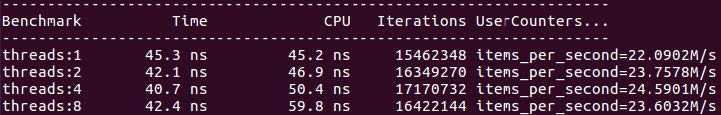
\includegraphics[width=0.9\textwidth]{content/2/chapter7/images/15.jpg}\\ 
圖7.15 —— x86 CPU上無鎖堆棧的性能(與圖7.11相比)
\end{center}

為了進行比較,自旋鎖保護的堆棧可以在同一臺機器上每秒執行大約70M個操作。這與前一節對性能評估的預期一致。然而,同樣的評估表明,無鎖堆棧可能優於ARM處理器。基準測試證明瞭我們的努力沒有白費:

%\hspace*{\fill} \\ %插入空行
\begin{center}
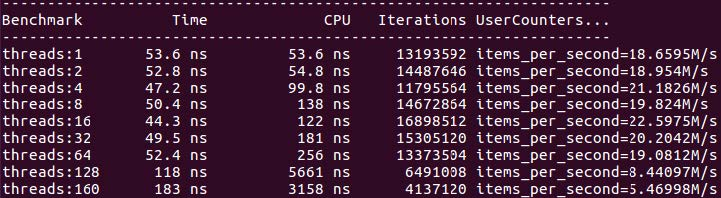
\includegraphics[width=0.9\textwidth]{content/2/chapter7/images/16.jpg}\\ 
圖7.16 - ARM CPU上無鎖堆棧的性能(與圖7.12相比)
\end{center}

基於鎖的堆棧單線程性能更好,如果線程數量大,則無鎖堆棧的速度要快得多。如果基準測試包含大量的\texttt{top()}調用(許多線程在一個線程拋出頂層元素之前讀取了它),或者如果生產者和消費者線程是不同的(一些線程只使用\texttt{push()},而其他線程只使用\texttt{pop()}),那麼無鎖堆棧的優勢就會更大。

本節中,我們研究了線程安全堆棧數據結構的不同實現。為了理解線程安全需要什麼,必須分別分析每個操作,以及多個併發操作的交互。以下是我們得到的經驗:

\begin{itemize}
\item 
有了好的鎖實現,鎖保護的堆棧提供了合理的性能,並且比其他選擇簡單得多。

\item 
關於數據結構的使用,限制特定於應用程序的信息,都應該用來以較低的成本獲得較好的性能。但這不是開發通用解決方案的地方,而實現儘可能少的特性,並試圖從限制中獲得性能優勢才是要做的事情。

\item 
通用的無鎖實現是可能的,但對於像堆棧這樣簡單的數據結構,也相當複雜。有時,這種複雜性甚至是合理的。

\end{itemize}

目前為止,我們還沒有討論到內存管理的問題。當堆棧耗盡容量時,它隱藏在分配更多內存的後面。我們稍後會再回到這個問題上的。這裡,先讓我們探索一下其他的數據結構。


































